\documentclass[../sparc.tex]{subfiles}
\graphicspath{{\subfix{../images/}}}
\begin{document}

%%%%%%%%%%%%%%%%%%%%%%%%%%%%%%%%%%%%%%%%%%%%%%%%%%%%%%%%%%%%%%%%%%%%%%%%%%%%%%%%
\subsection{Шина I2C}
\label{section:i2c}
\index{Электроника!Шина I2C}
\newglossaryentry{I2C}{name=I2C, description={Inter-Integrated Circuit}}

\newglossaryentry{USB}{name=USB, description={Universal Serial Bus --
    ``Универсальная последовательная шина.''}}

\newglossaryentry{PCI}{name=PCI, description={Peripheral component interconnect
    -- ``взаимосвязь периферийных компонентов''}}

\newglossaryentry{I/O}{name=I/O, description={I/O -- ``Input/Output''}}

\textit{\gls{I2C}} также иногда называемя $I^{2}C$ (читается ``ай-квадрат-си''),
-- шина передачи данных, используемая для связи между интегральными схемами
внутри электронных приборов. Давайте рассмотрим во-первых, что такое ``шина
передачи данных''. Если кратко, то \textit{шина} (англ. \textit{bus}) в
архитектуре компьютера -- это некое соединение, служащее для передачи данных
между функциональными блоками коммьютера.

Шины передачи данных условно можно разделить на две крупные категории --
\textit{внешние} шины и \textit{внутренние} шины.

К внешним шинам можно отнести наверняка знакомый многим из вас \gls{USB} --
данная шина используется для соединения внешних устройств (таких, как Arduino,
клавиатура, мышь, принтер и т.п.) с компьютером.  Подобные шины как правило
имеют стандартизированный разъём и достаточно большую длину провода.

К внутренним шинам относится уже упомянутый выше \gls{I2C} и \gls{PCI}/PCI
Express (используемой например для подключения сетевой карты к материнской плате
компьютера.  Внутренние шины обычно подразумевают передачу данных на короткие
дистации, оперативное отключение/подключение компонентов не предусмотрено и,
следовательно, некоторые из внутренних шин не имеют своего специализированного
разъёма и бывают просто распаены прямо на плате.

Максимальная длина соединения между компонентами на шине \gls{I2C} не должна
превышать 30 сантиметров, в противном случае данные будут передаваться
ненадёжно.

\gls{I2C} имеет достаточно низкую скорость передачи данных (не более 5МБит/с)
между устройствами. У каждого устройства есть свой \textit{адрес} на шине --
можно сказать, его поядковый номер. На одну шину можно подключить до 127
устройств с уникальными адресами. При этом, на шине одно устройство является
ведущим (как правило, это какой-либо микроконтроллер) и остальные устройства
являются ведомыми.

На рис. \ref{fig:i2c-schematics} показана схема шины \gls{I2C}. Как можно видеть
на рисунке, шина использует всего две линии для передачи данных -- ``Serial Data
Line'' (\textbf{SDL}) и ``Serial Clock Line'' (\textbf{SCL}). Обе линии
подтянуты через резисторы \textbf{$R_p$} к напряжению питания (\textbf{Vdd}). На
схеме ``$\mu$C\\Controller'' -- это ведущее устройство, остальные же, указанные как
``Target'', являются ведомыми.

Большинство ЖК-дисплеев имеют уже припаянный к нему \gls{I2C}-модуль, либо же
подобный модуль можно купить и припаять отдельно.  Как правило основой такого
модуля выступает специальная микросхема -- \gls{I/O}-расширитель PCF8574.

Некоторые модели дисплеев изначально имеют I2C-интерфейс и отдельного модуля для
них не требуется, так как необходимая ``обвязка'' уже распаяна прямо на плате
дисплея.

\begin{figure}[H]
  \centering
  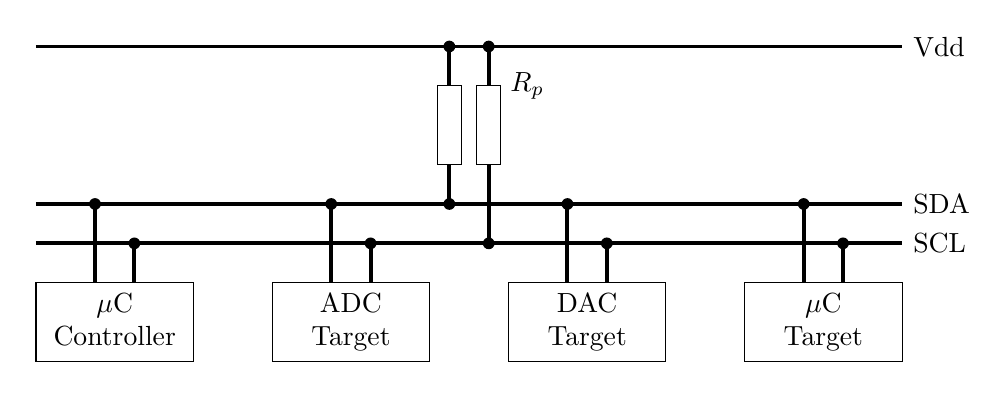
\begin{tikzpicture}
    \draw[draw=black] (0, 2) rectangle ++(2, 1) node[pos=.5] {%
      \begin{tabular}{c}%
        $\mu$C\\Controller%
    \end{tabular}};
    \draw[draw=black] (3, 2) rectangle ++(2, 1) node[pos=.5] {
      \begin{tabular}{c}
        ADC\\Target
    \end{tabular}};
    \draw[draw=black] (6, 2) rectangle ++(2, 1) node[pos=.5] {
      \begin{tabular}{c}
        DAC\\Target
    \end{tabular}};
    \draw[draw=black] (9, 2) rectangle ++(2, 1) node[pos=.5] {
      \begin{tabular}{c}
        $\mu$C\\Target
    \end{tabular}};

    %% Horizontal lines.
    \draw [line width=0.5mm] (0, 3.5) -- (11, 3.5) node[right] {SCL};
    \draw [line width=0.5mm] (0, 4.0) -- (11, 4.0) node[right] {SDA};
    \draw [line width=0.5mm] (0, 6.0) -- (11, 6.0) node[right] {Vdd};

    %% Vertical lines.
    \foreach \a/\b in {0.75/1.25, 3.75/4.25, 6.75/7.25, 9.75/10.25} {
      \draw [line width=0.5mm] (\a, 3) -- (\a, 4) node[circle,fill,inner sep=1.5pt]{};
      \draw [line width=0.5mm] (\b, 3) -- (\b, 3.5) node[circle,fill,inner sep=1.5pt]{};
    };

    \draw[line width=0.5mm] (5.25, 4) node[circle,fill,inner sep=1.5pt]{}
    -- (5.25, 6) node[circle,fill,inner sep=1.5pt]{};
    \draw[line width=0.5mm] (5.75, 3.5) node[circle,fill,inner sep=1.5pt]{}
    -- (5.75, 6) node[circle,fill,inner sep=1.5pt]{};

    \draw[draw=black, fill=white] (5.1, 4.5) rectangle ++(0.3, 1);
    \draw[draw=black, fill=white] (5.6, 4.5) rectangle ++(0.3, 1) node[right] {$R_p$};

  \end{tikzpicture}
  \caption{Устройство шины \gls{I2C}.}
  \label{fig:i2c-schematics}
\end{figure}

\end{document}
